\chapter{Digr\'aficas de intervalos ajustadas}
\label{cap:DigrafIntAj}

\section{Digr\'aficas de intervalos}

En el año 1989 se public\'o un articulo de M. Sen, S. Das, A.B. Roy y D.B. West
en el  \textit{Journal of Graph Theory}. En este se introduce una nueva
definici\'on que generaliza a las gr\'aficas de intervalos. Dicha
generalizaci\'on iba enfocada a tener caracterizaciones an\'alogas a las de las
gr\'aficas de intervalos, una de ellas, la propiedad de los unos consecutivos
para columnas de la matriz asociada a la gr\'afica de clanes maximales.
Desafortunadamente esta definici\'on, no cuenta con un alguna caracterizaci\'on
en t\'erminos de estructuras prohibidas, como sí las tienen las gr\'aficas de
intervalos, en t\'erminos de las tripletas asteroidales y $k$-ciclos sin
cuerdas, $k \geq 4$. Así, al solo contar con una caracterizaci\'on sencilla, a
saber, a trav\'es de la propiedad de los unos consecutivos, el único algoritmo
de reconocimiento para esta clase no es eficiente.

En el artículo arriba mencionado, se define una digr\'afica de intervalos como
una digr\'afica $G$ la cual admite una representaci\'on de pares de intervalos,
es decir, para cada v\'ertice $v \in V(G)$, existen $I_v,J_v$ un par de
intervalos, y $uv\in E(G)$ si y solo si $I_u$ intersecta a $J_v$. 

En el \'animo de explorar las propiedades de las digr\'aficas de intervalos
surge una pregunta muy natural. ¿Puede una digr\'afica, cuya gr\'afica
subyacente no sea una gr\'afica de intervalos, ser una digr\'afica de
intervalos? La respuesta puede responderse inmediatamente mediante este primer
ejemplo. Comencemos con una digr\'afica muy sencilla, la cual se muestra en
\cref{fig:Dgrf01} y consta únicamente de dos v\'ertices, $v_1, v_2$, y que
carece de flechas, así como de lazos. Una representaci\'on por pares de
intervalos se muestra en la parte inferior, y es f\'acil comprobar que las
incidencias se respetan, pues los cuatro intervalos son ajenos dos a dos. Pero
en particular $I_1$ no intersecta a $J_1$ ni a $J_2$ e $I_2$ tampoco intersecta
a $J_1$ o a $J_2$. Para responder la pregunta, hacemos la siguiente nota, en la
definici\'on de las gr\'aficas de intervalos es implícito que las gr\'aficas
cuenten con lazos, mas aún que sean reflexivas. Como primer contraste, en el
caso dirigido se pierde esto, como se mostr\'o en el presente ejemplo. Así que
el hecho de que la gr\'afica suyacente no sea gr\'afica de intervalos no nos
arroja mayor informaci\'on. 

\begin{figure}[H]
  \centering
  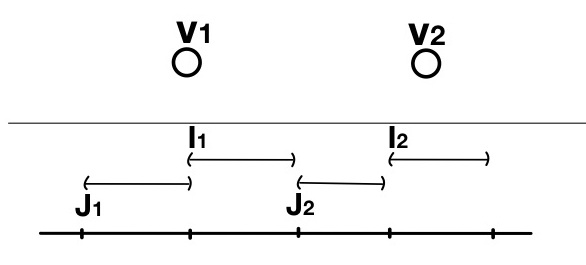
\includegraphics[width=0.5\textwidth]{recursos/capturas/Digraf1.jpg}
  \caption{Digr\'afica sin flechas ni lazos.}
  \label{fig:Dgrf01}
\end{figure}


Ahora vemos que al añadir una flecha que sale de $v_1$ a $v_2$ nosotros seguimos
teniendo que esta digr\'afica tiene una representaci\'on por pares de
intervalos. Para dar la representaci\'on, podemos usar como base la que se dio
en la imagen anterior y solo modificar los intervalos $I_1,J_2$; debemos buscar
que $I_1\cap J_2 \neq \emptyset$, es decir, que tengan intersecci\'on no vacía,
ya que queremos rescatar el hecho de tener la flecha $(v_1,v_2)$. Para lograr
esto, basta extender un poco hacia la derecha el extremo derecho del intervalo
$I_1$. 

\begin{figure}[H]
  \centering
  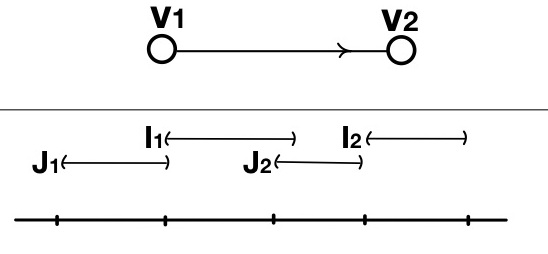
\includegraphics[width=0.5\textwidth]{recursos/capturas/Digraf2.jpg}
  \caption{Digr\'afica con una sola flecha.}
  \label{fig:Dgrf02}
\end{figure}


A continuaci\'on en \cref{fig:Dgrf03} se muestra que al añadir la flecha en el
otro sentido se sigue teniendo una representaci\'on de pares de intervalos y por
tanto se tiene que nuevamente es digr\'afica de intervalos. Para verificar esto,
comenzamos haciendo una pequeña modificaci\'on a la representaci\'on de pares de
la figura anterior. En primer lugar situamos el intervalo $I_2$ a la izquierda
de todos los intervalos y extendemos el extremo derecho del intervalo de tal
forma que este intersecte al intervalo $J_1$.

\begin{figure}[H]
  \centering
  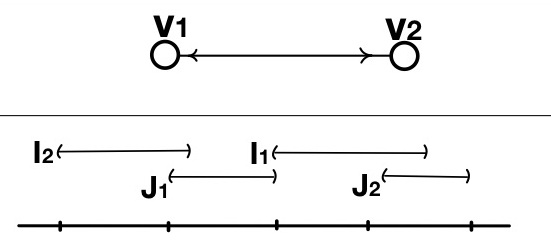
\includegraphics[width=0.5\textwidth]{recursos/capturas/Digraf3.jpg}
  \caption{Digr\'afica con dos flechas.}
  \label{fig:Dgrf03}
\end{figure}

Finalmente exhibimos que al añadir todas las posibles flechas y lazos en el
ejemplo dado en \cref{fig:Dgrf01} seguimos teniendo una digr\'afica de
intervalos. Tomamos la representaci\'on del ejemplo anterior y para añadir el
lazo en $v_1$ tenemos que $I_1$ debe intersecar a $J_1$ y an\'alogamente tenemos
que hacer que $I_2$ intersecte a $J_2$ para así tener el lazo en $v_2$. N\'otese
que $I_1$ e $I_2$ pueden o no intersectarse pues esto no afecta a las flechas,
aquí los ponemos disjuntos.

\begin{figure}[H]
  \centering
  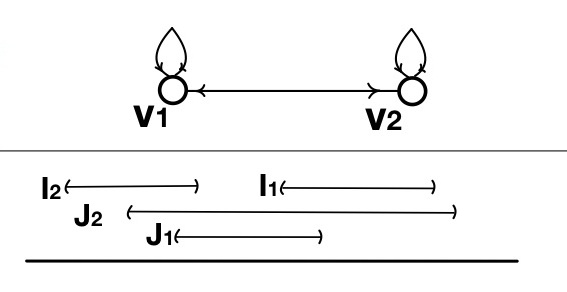
\includegraphics[width=0.5\textwidth]{recursos/capturas/Digraf4.jpg}
  \caption{Digr\'afica de dos v\'ertices y todas las flechas y lazos posibles.}
  \label{fig:Dgrf04}
\end{figure}
 
Como se vio desde nuestro primer ejemplo, una digr\'afica de intervalos puede
tener como subgr\'afica subyacente una gr\'afica la cual no sea de intervalos,
como el siguiente ejemplo, el cual tiene como gr\'afica subyancete un 4-ciclo el
cual se vio que no es gr\'afica de intervalos. 

Ante la ausencia de una caracterizaci\'on en t\'erminos de estructuras
prohibidas sencillas de las digr\'aficas de intervalos, Tom\'as Feder, Pavol
Hell, Jing Huang y Arash Rafiey, publicaron un artículo en 2011 donde introducen
una pequeña modificaci\'on a las digr\'aficas de intervalos, dando pie a la
definici\'on de digr\'afica de intervalos ajustada.

%%%%%%%%%%%%%%%%%%%%%%%%%%%%%%%%%%%%%%%%%%%%%%%%%%%%%%%%%%%%%%%%%%%%%%%%%%%%%%%%%%%%%
%%%%%%%%%%%%%%%%%%%%%%%%%%%%%%%%%%%%%%%%%%%%%%%%%%%%%%%%%%%%%%%%%%%%%%%%%%%%%%%%%%%%%
%%%%%%%%%%%%%%%%%%%%%%%%%%%%%%%%%%%%%%%%%%%%%%%%%%%%%%%%%%%%%%%%%%%%%%%%%%%%%%%%%%%%%
%%%%%%%%%%%%%%%%%%%%%%%%%%%%%%%%%%%%%%%%%%%%%%%%%%%%%%%%%%%%%%%%%%%%%%%%%%%%%%%%%%%%%
%%%%%%%%%%%%%%%%%%%%%%%%%%%%%%%%%%%%%%%%%%%%%%%%%%%%%%%%%%%%%%%%%%%%%%%%%%%%%%%%%%%%%

\section{Digr\'aficas de intervalos ajustadas}

Una digr\'afica de intervalos ajustada $G$ es una digr\'afica de intervalos $G$
la cual tiene una representaci\'on por pares de intervalos $I_v, J_v$ para cada
$v\in V(G)$ de tal forma que $I_v$ y $J_v$ tienen el mismo extremo izquierdo. 

Con este pequeño ajuste, uno vuelve a recuperar la parte de la reflexividad, ya
que $I_v,J_v$ tienen el mismo extremo izquierdo, entonces son no ajenos, luego
se debe tener que $(v,v)\in E(G)$. Al mismo tiempo con esta modificaci\'on
saldr\'a a relucir una estructura prohibida para esta nueva clase de
digr\'aficas.

Ahora exploremos unos ejemplos, claramente \crefrange{fig:Dgrf01}{fig:Dgrf03} no
pueden ser digr\'aficas de intervalos ajustadas, ya que son no reflexivas.
Entonces veamos si al ponerles todos los lazos estas cumplen ser digr\'aficas de
intervalos ajustadas.

En el primer caso al añadir los lazos, se tiene la representaci\'on de pares de
intervalos, cuyos pares de intervalos correspondientes a $v$ tienen el mismo
extremo izquierdo. Por tanto, este constituye nuestro primer ejemplo de
digr\'afica de intervalos ajustada.

\begin{figure}[H]
  \centering
  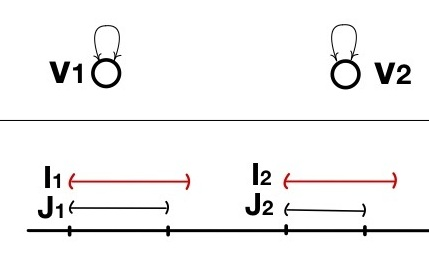
\includegraphics[width=0.4\textwidth]{recursos/capturas/Dgrf_Int_Adj01.jpg}
  \caption{Digr\'afica de intervalos ajustada. Dos v\'ertices y sin flechas salvo lazos.}
  \label{fig:DgrfAdj01}
\end{figure}

En el segundo ejemplo, se puede encontrar nuevamente una representaci\'on por
pares de intervalos que satisfaga el ajuste planteado por Tom\'as Feder et al. 

\begin{figure}[H]
  \centering
  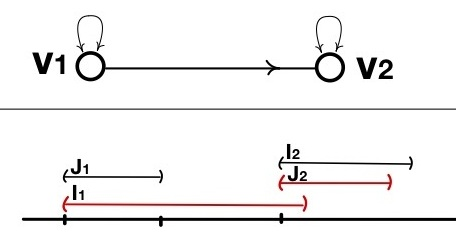
\includegraphics[width=0.45\textwidth]{recursos/capturas/Dgrf_Int_Adj02.jpg}
  \caption{Digr\'afica de intervalos ajustada. Dos v\'ertices, una flecha.}
  \label{fig:DgrfAdj02}
\end{figure}

Finalmente, si agregamos la flecha $(v_2, v_1)$ entonces damos la siguiente
representaci\'on ajustada por pares de intervalos. 

\begin{figure}[H]
  \centering
  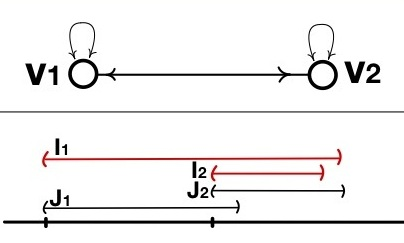
\includegraphics[width=0.4\textwidth]{recursos/capturas/Dgrf_Int_Adj03.jpg}
  \caption{Digr\'afica de intervalos ajustada con dos v\'ertices y dos flechas.}
  \label{fig:DgrfAdj03}
\end{figure}

A continuaci\'on introducimos definiciones muy sencillas. Dado un camino
$P=x_0,\dots,x_n$ en una digr\'afica $G$ y $u,v \in V(G)$ tales que constituyan
una flecha, es decir $(u,v) \in E(G)$ o $(v,u) \in E(G)$ decimos que  $(u,v)$ es
una flecha derecha si $(u,v) \in E(G)$ y decimos que es una flecha al rev\'es si
$(v,u) \in E(G)$. En \cref{fig:DgrfAdj02} podemos decir entonces que $(v_1,v_2)$
es una flecha derecha porque precisamente $(v_1,v_2) \in E(G)$. De forma
similar, $(v_2,v_1)$ es una flecha al rev\'es. Sin embargo, uno ve
\cref{fig:DgrfAdj03} y se pregunta qu\'e pasa respecto a $(v_1,v_2)$, a estas
flechas las cuales sean tanto derechas como al rev\'es, las llamaremos flechas
dobles. Aquellas flechas que no son dobles, como la que se muestra en
\cref{fig:DgrfAdj02}, se pueden llamar flechas únicamente derechas o únicamente
al rev\'es, según sea el caso. Naturalmente los lazos al ser flechas derechas y
al rev\'es, son flechas dobles. Si $(u,v)\in E(G)$ diremos que $u$ domina a $v$
o que $v$ es dominado por $u$, sin importar si $(u,v)$ es una flecha doble o
única. Esto llevado nuevamente a \cref{fig:DgrfAdj02}, podemos decir entonces
que $v_1$ domina a $v_2$. Estas definiciones nos permiten introducir el concepto
de caminos congruentes. Dos caminos $P=x_0, \dots, x_n$ y $Q=y_0, \dots, y_n$ en
$G$ se dice que son congruentes si tienen el mismo patr\'on de flechas derechas
y al rev\'es, esto es $P,Q$ son caminos congruentes si y solo si $(
x_i,x_{i+1})$ es flecha derecha si y solo si $(y_i, y_{i+1})$ es flecha derecha,
para toda $0\leq i \leq n-1 $.

\begin{figure}[H]
  \centering
  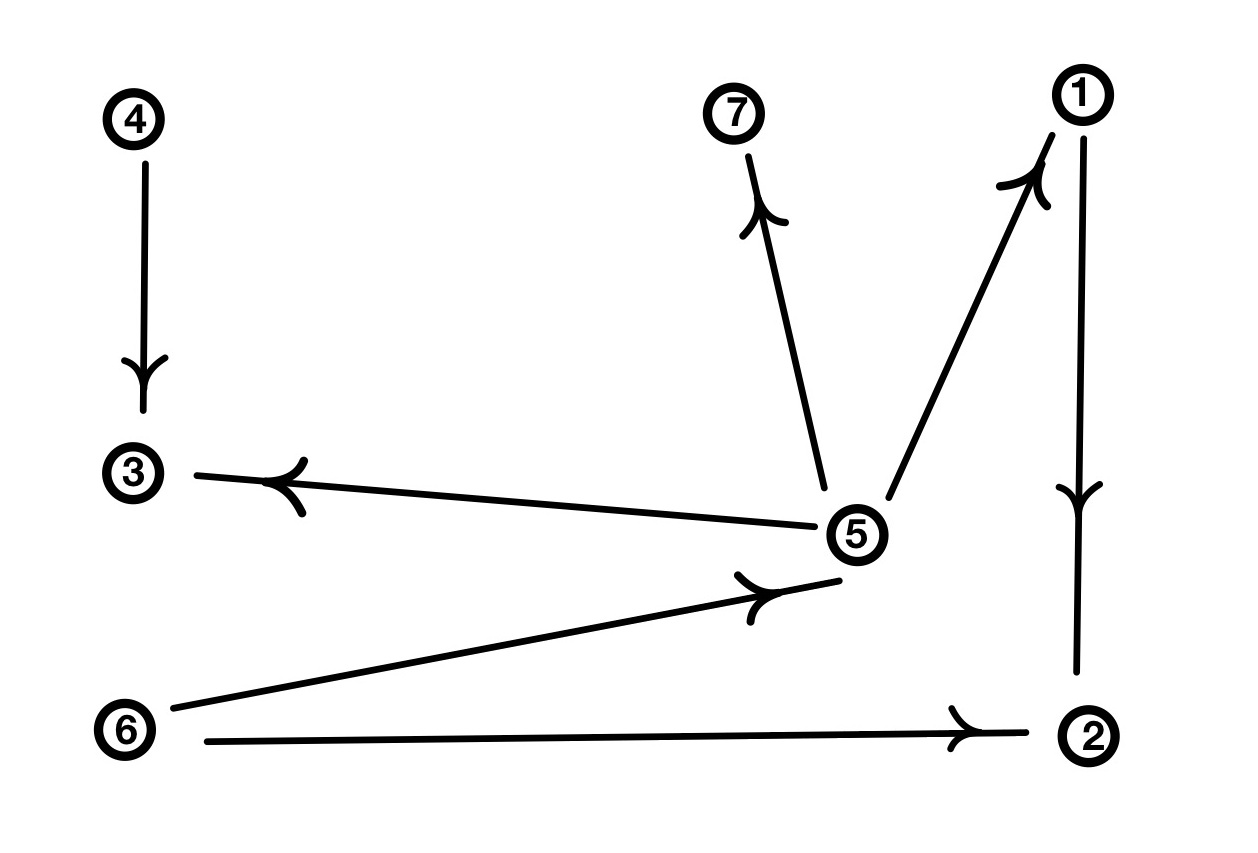
\includegraphics[width=0.4\textwidth]{recursos/capturas/CaminoCngrnt.jpg}
  \caption{Caminos $P=(1,2,6,5,7)$ y $Q=(4,3,5,1,2)$ congruentes.}
  \label{fig:CaminoCngrnt}
\end{figure}

En \cref{fig:CaminoCngrnt} se puede observar un par de camino congruentes
$P=(1,2,6,5,7)$ y $Q=(4,3,5,1,2)$. Ahora introducimos una siguiente
definici\'on, dados un par de caminos congruentes $P$ y $Q$, decimos que $P$
evita a $Q$ si y solo si no hay flechas $(x_i,y_{i+1})$ en la misma
orientaci\'on que las flechas $(x_i,x_{i+1})$. En el ejemplo anterior podemos
afirmar que $P$ evita a $Q$, sin embargo, $Q$ no evita a $P$, ya que la flecha
$(5,1)$ es derecha y la flecha $(5,5)$ al ser una flecha doble en particular es
derecha y luego, $Q$ no evita a $P$.

\begin{figure}[H]
  \centering
  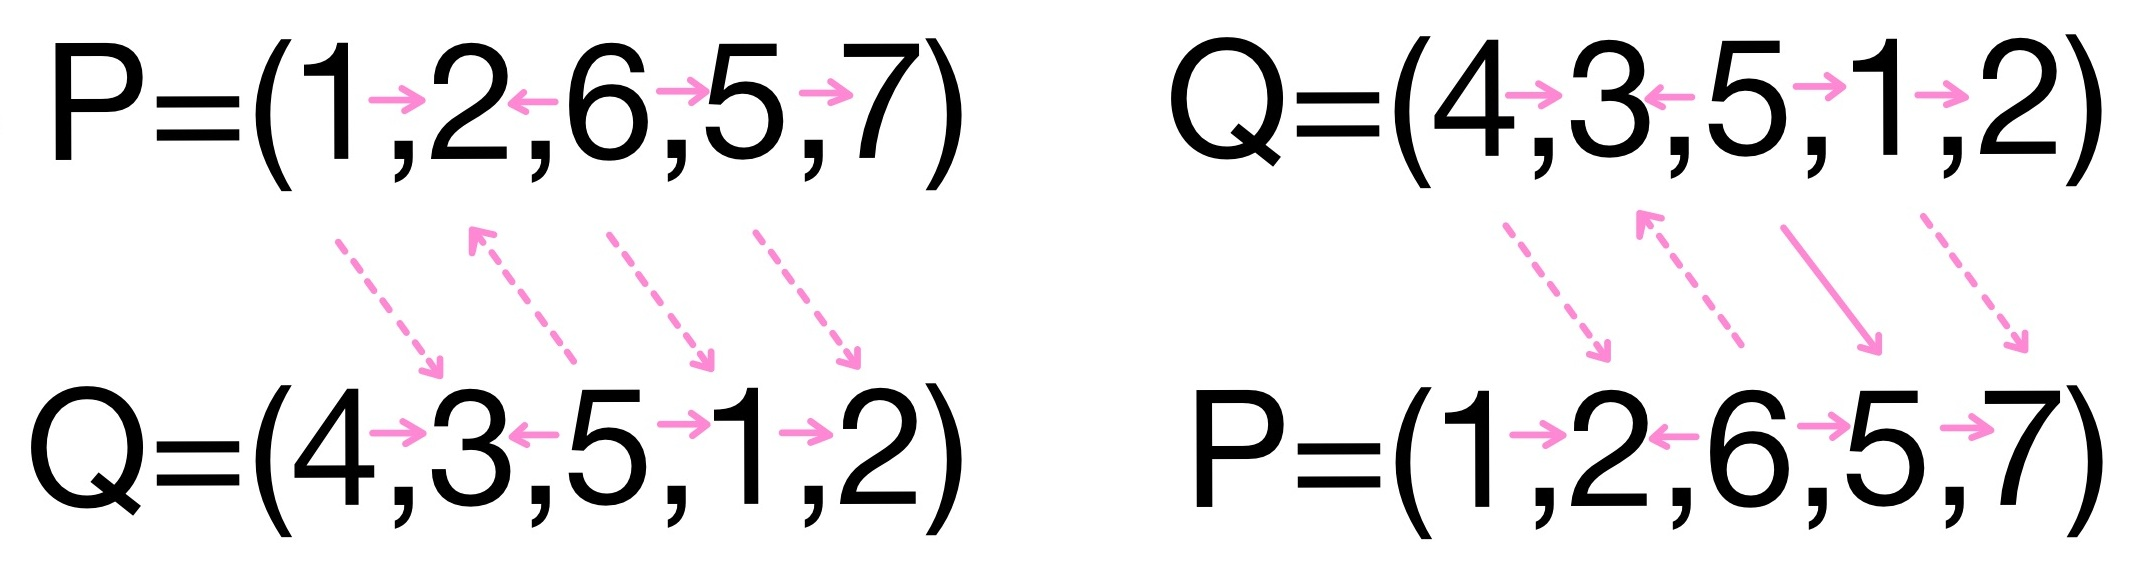
\includegraphics[width=0.5\textwidth]{recursos/capturas/Esqm.jpg}
  \caption{En este esquema las lineas punteadas son flechas que no pertenecen a $E(G)$, así a la izquierda se observa que $P$ evita a $Q$, a la derecha al se verifica que $Q$ no evita a $P$.}
  \label{fig:Esqm}
\end{figure}

Con todo lo anterior podemos dar paso a la definici\'on de \indice{par
invertible}, estructura la cual nos permitir\'a caracterizar a las digr\'aficas
de intervalos ajustadas. Un par invertible en una digr\'afica $G$ es un par de
v\'ertices $u,v \in V(G)$ tales que cumplen, en primer lugar, que existen
caminos congruentes $P$ de $u$ a $v$ y $Q$ de $v$ a $u$ de tal forma que $P$
evita a $Q$, y en segundo lugar, que existen caminos congruentes $P'$ de $v$ a
$u$ y $Q'$ de $u$ a $v$, de tal forma que $P'$ evita a $Q'$.

A continuaci\'on damos un par de ejemplos de digr\'aficas que tienen pares
invertibles. Para nuestro primer ejemplo damos el $4$-ciclo $(1,2,3,4,1)$.
Afirmamos que en esta digr\'afica los v\'ertices $1$ y $3$ constituyen nuestro
par invertible. Para esto damos los caminos congruentes $P=(1,2,3), Q=(3,4,1)$,
notemos que así definidos los caminos son congruentes, tal y como se ilustra en
el esquema de la derecha del $4$-ciclo de \cref{fig:InvrtblPair01} y adem\'as
$P$ evita a $Q$ (las flechas en gris no pertenecen a $E(G)$). Recordando nuestra
definici\'on, necesitamos ahora otro par de caminos congruentes $P'$ y $Q'$,
estos los definimos de la siguiente manera $P'=(3,2,1), Q'=(1,4,3)$ nuevamente
usando el esquema de \cref{fig:InvrtblPair01}, se comprueba que dichos caminos
son congruentes y que adem\'as $P'$ evita a $Q'$.

\begin{figure}[H]
  \centering
  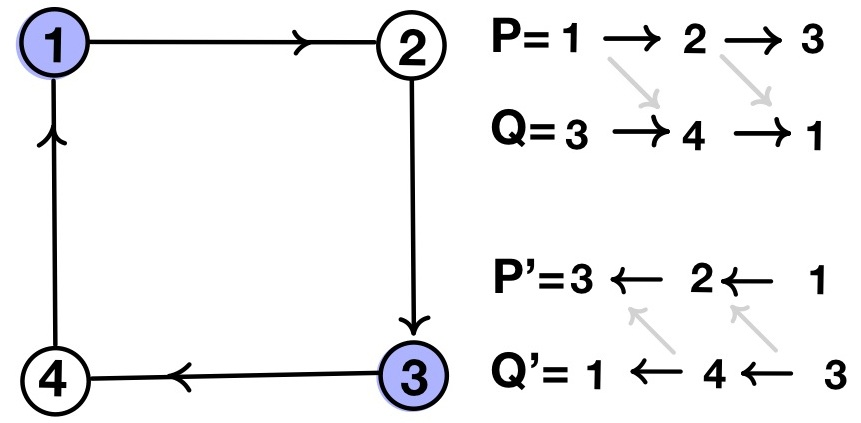
\includegraphics[width=0.5\textwidth]{recursos/capturas/InvtblPair01.jpg}
  \caption{Los v\'ertices azules constituyen un par invertible. A la derecha los caminos congruentes $P,Q$, $P',Q'$.}
  \label{fig:InvrtblPair01}
\end{figure}

Un hecho interesante del ejemplo anterior es que es posible definir a $P'$ y a
$Q'$ como los caminos inversos de $P$ y $Q$ respectivamente, donde entendemos
que dado un camino $(x_0,x_1, \dots, x_n)$ el camino inverso es $(x_n,x_{n-1},
\dots, x_0)$. Aunque esto no se puede hacer en general, en este caso, la validez
de lo anterior se debe a que tanto $P$ evita a $Q$ como $Q$ evita a $P$. 

A continuaci\'on hacemos sim\'etricas las flechas de la gr\'afica anterior para
tener un ejemplo donde es imposible definir a $P', Q'$ como los caminos inversos
de $P, Q$ respectivamente. Veamos \cref{fig:InvrtblPair02}. Nuevamente tenemos
que los v\'ertices $1$ y $3$ son un par invertible. Algo importante a destacar
es que los pares de caminos del ejemplo pasado, si bien siguen siendo
congruentes, dejan de evitarse. Por ejemplo para que $P$ evite a $Q$ necesitamos
que $(1,4),(2,1)\notin E(G)$, algo que no sucede en el presente ejemplo. Por lo
anterior es necesario dar otro par de caminos $P$ y $Q$. Definimos
$P=(1,2,2,3,3)$ y $Q=(3,3,4,4,1)$. Así definidos los caminos, son congruentes y
adem\'as $P$ evita a $Q$. Si uno tratara de definir los caminos $P'$ y $Q'$ como
los caminos inversos de $P$ y $Q$ respectivamente, uno caería en cuenta que así
definidos el camino $P'$ no evita a $Q'$. Por lo que debemos encontrar otra
forma alterna para definir a $P'$ y a $Q'$. Así, damos $P'=(3,4,4,1,1)$ y
$Q'=(1,1,2,2,3)$ y definidos de esta forma, $P', Q'$ son caminos congruentes y
son tales que $P'$ evita a $Q'$.

\begin{figure}[H]
  \centering
  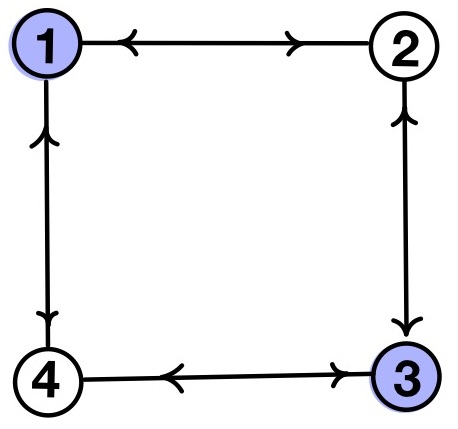
\includegraphics[width=0.5\textwidth]{recursos/capturas/InvrtblPair02.jpg}
  \caption{Los v\'ertices azules constituyen un par invertible.}
  \label{fig:InvrtblPair02}
\end{figure}

En los ejemplos pasados se puede verificar mediante argumentos sim\'etricos que
los v\'ertices $2,4$ son tambi\'en pares invertibles. 

A continuaci\'on definiremos una digr\'afica auxiliar, en la cual se rescata
bastante informaci\'on respecto a todos los pares invertible de una gr\'afica
$G$, en caso de que existan. Dada una digr\'afica $G$, definimos la digr\'afica
de pares asociada a $G$, denotada por $G^{+}$ la cual est\'a definida como
$V(G^{+})=\{ (u,v)\in G\times G \colon\ u\neq v \}$ y diremos que
$((u,v),(u',v'))\in F(G^{+})$ si y solo si sucede una de las siguientes dos
cosas; $(u,u'),(v,v')\in E(G)$ y $(u,v')\notin E(G)$ o si sucede que
$(u',u),(v',v)\in E(G)$ y $(v',u)\notin E(G)$. Usemos como ejemplo
\cref{fig:InvrtblPair01} para dar la digr\'afica de pares asociada.

\begin{figure}[H]
  \centering
  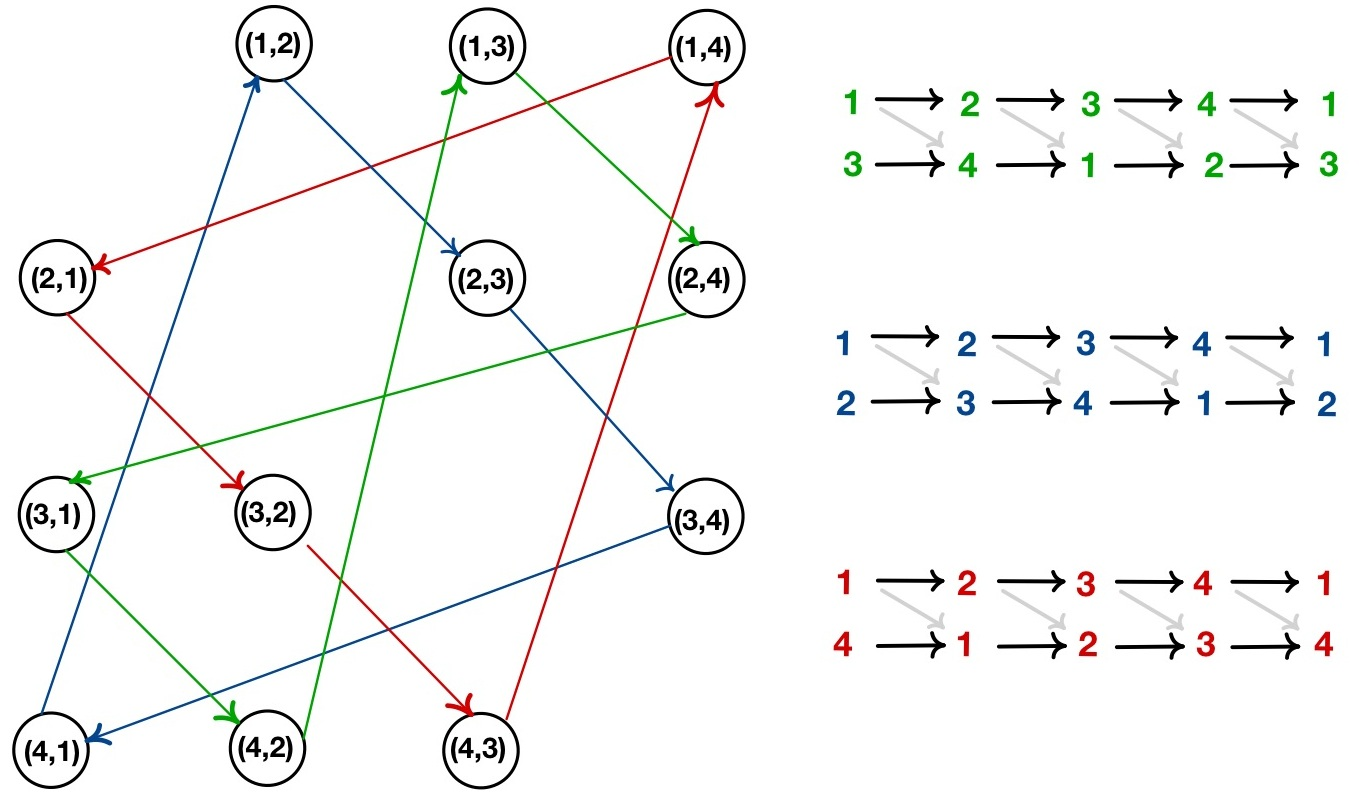
\includegraphics[width=0.75\textwidth]{recursos/capturas/PairDgrph.jpg}
  \caption{Los colores distintos corresponden a las componentes fuertes de $G^+$.}
  \label{fig:InvrtblPair02}
\end{figure}

Apoy\'andonos del esquema de la derecha, podemos verificar que en efecto las
flechas que est\'an dibujadas, son flechas según la definici\'on de las flechas
de la digr\'afica de pares. Coloreamos de colores distintos las tres componentes
fuertes distintas. Como hicimos notar, la pareja de v\'ertices $2,4$ tambi\'en
constituye un par invertible, algo interesante es el hecho que los v\'ertices
$(1,3)$ y  $(2,4)$ pertenecen a la misma componente fuerte (verde). El siguiente
teorema nos dice m\'as sobre esta interesante observaci\'on y tambi\'en arroja
m\'as informaci\'on sobre el resto de v\'ertices y las componentes conexas.

\begin{teorema}
\label{teo:PairDigrph}
    Supongamos que $u$ y $v$ forman un par invertible de la digr\'afica $G$.
    Entonces $(u,v)$ y $(v,u)$ pertenecen a la misma componente fuertemente
    conexa $C$ de la digr\'afica de pares $G^+$. M\'as aún, cualquier otra
    pareja $(x,y)$ que pertenezca a $C$, cumple que su par revertido $(y,x)$ es
    tambi\'en elemento de $C$.  Como consecuencia, si $(x,y) \in C$ entonces
    $x,y$ es un par invertible. Por otro lado si $H$ no tiene pares invertibles,
    entonces por cada componente fuerte $C$ de $G^+$, existe una componente
    fuerte $C' \neq C$ tal que $(x,y)\in C $ si y solo si $(y,x)\in C'$
\end{teorema}


Antes de continuar con la prueba veremos otra cosa interesante que sucede en la
digr\'afica de pares $G^+$. Si tenemos que en $G^+$ hay un camino \textbf{P} de
$(u,v)$ a $(v,u)$ digamos \textbf{P}$=( (u,v), (x_1,y_1), \dots, (x_{n},y_n),
(v,u)) $ entonces en autom\'atico tendremos un par de caminos $P,Q$ congruentes,
$P=(u, x_1, \dots, x_n,v)$ de $u$ a $v$ y $Q=(v,y_1, \dots, y_n, u)$ de $v$ a
$u$ y que adem\'as $P$ evita a $Q$. De donde $P$ y $Q$ se obtienen al considerar
solo las primeras entradas del camino \textbf{P} y al considerar solamente las
segundas entradas del camino \textbf{P}, respectivamente. An\'alogamente, si
tambi\'en existe un camino en $G^+$ de $(v,u)$ a $(u,v)$, tendremos que existen
otro par de caminos $P',Q'$ congruentes, $P'$ de $v$ a $u$ y $Q'$ de $u$ a $v$
tales que $P'$ evita a $Q'$. Donde $P', Q'$ se construir\'an de forma similar a
como se construyeron $P$ y $Q$. Así, en el caso en el que hay un camino
\textbf{P} de $(u,v)$ a $(v,u)$ en $G^+$ y otro camino \textbf{Q} de $(v,u)$ a
$(u,v)$ en $G^+$, podremos afirmar que $u,v$ constituyen un par invertible de
$G$. 

\begin{proof}
    Probemos como primer punto que si $u,v$ son un par invertible, entonces
    $(u,v)$ y $(v,u)$ pertenecen a la misma componente fuertemente conexa. Ahora
    veamos que si $(x,y)\in C$ entonces $(y,x)\in C$. Para esto haremos una
    primera nota, $((u,v),(u',v'))\in E(G^+)$ implica que $((v',u'),(v,u))\in
    E(G^+)$, esto se puede corroborar observando \cref{fig:FlechaRevertida}.
    Ahora sí, continuemos con la prueba, como $(x,y) \in C$ entonces la reversa
    de un camino cerrado que contiene a $(u,v),(x,y)$ (usando la observaci\'on)
    es un camino cerrado que contiene a $(v,u),(y,x)$.    Luego, por
    concatenaci\'on de estos caminos cerrados, obtenemos otro camino cerrado que
    contiene a $(u,v),(v,u)$ y así podemos concluir que $(x,y),(y,x)$ pertenecen
    a la misma componente fuerte $C$. Esto se puede observar en
    \cref{fig:RvrtdPath}. Finalmente si no existe un par invertible, para cada
    $(x,y)$ sabemos que $(y,x)$ no pertenece a la misma componente de $(x,y)$
    pues en ese caso $x,y$ en efecto constituye un par invertible. Luego para
    cada $(x,y)\in C$ existe una componente $C'$ tal que $(y,x)\in C'$. 
\end{proof}

\begin{figure}[H]
  \centering
  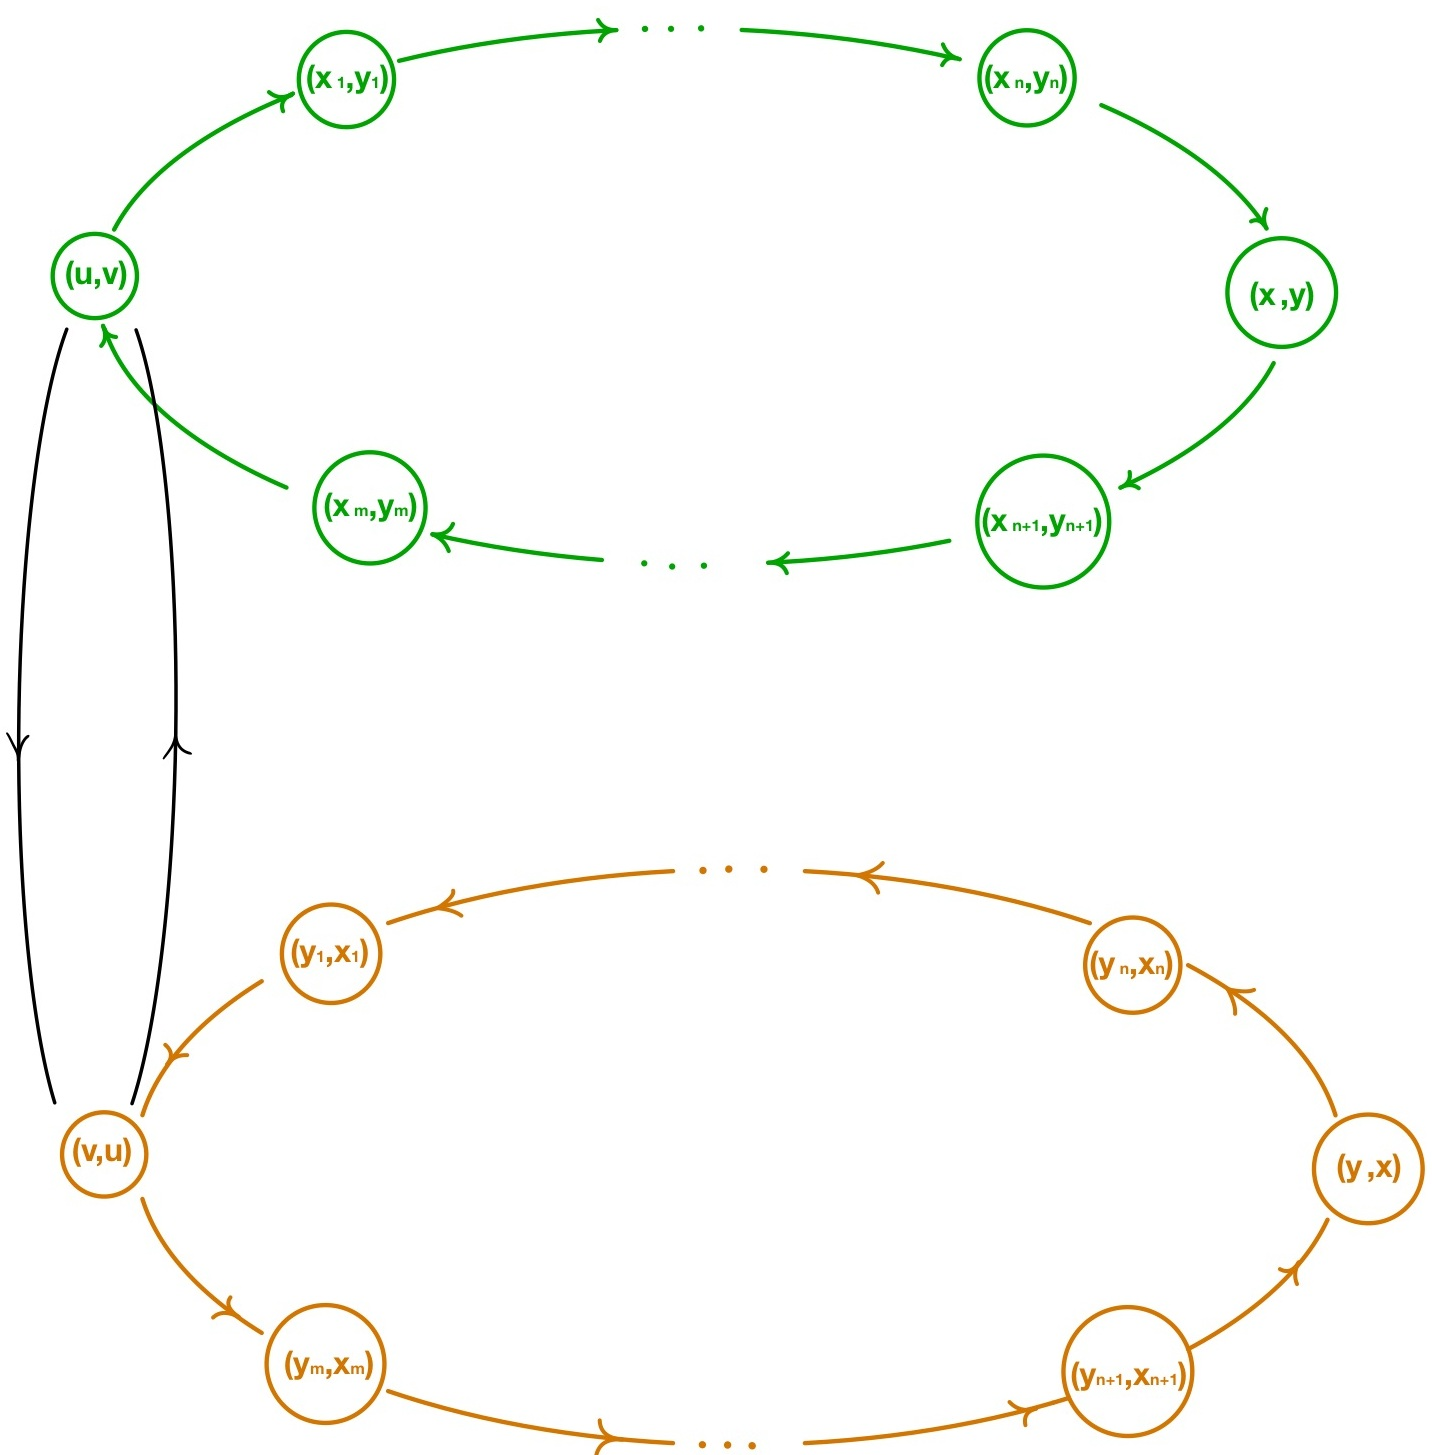
\includegraphics[width=0.65\textwidth]{recursos/capturas/RvrtdPath.jpg}
  \caption{En verde el camino cerrado que contiene a $(u,v),(x,y)$. En naranja el camino revertido del camino verde. Al seguir el sentido de las flechas se obtiene un camino que contiene a $(uv),(v,u)$ }
  \label{fig:RvrtdPath}
\end{figure}

\begin{figure}[H]
  \centering
  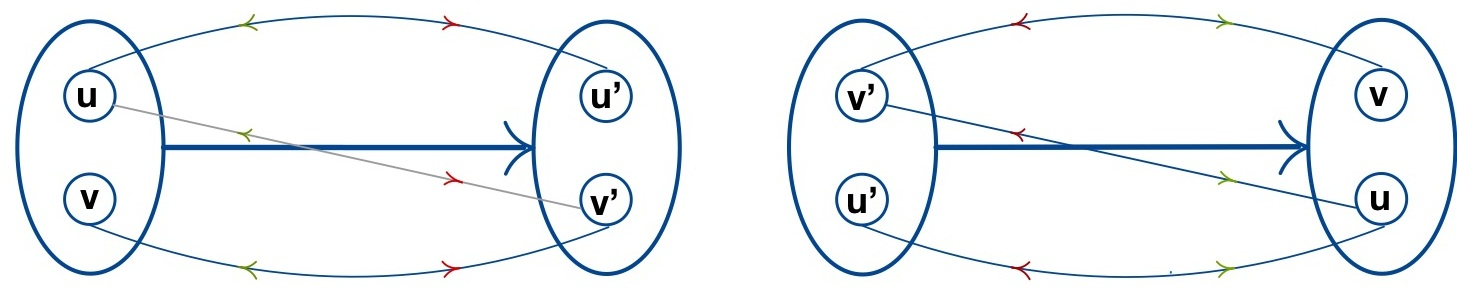
\includegraphics[width=0.85\textwidth]{recursos/capturas/(uv,u'v').jpg}
  \caption{Si $(uv,u'v')\in E(G^+)$ entonces $(v'u',vu)\in E(G^+)$. Representamos en color verde y rojo las flechas de los dos casos distintos que se obtiene cuando $(uv,u'v')\in E(G^+)$. En color gris representamos una flecha que no pertenece a $E(G)$.}
  \label{fig:FlechaRevertida}
\end{figure}

En el siguiente teorema, exhibimos un nuevo concepto, el de ordenamiento mínimo.
M\'as adelante veremos que este concepto esta íntimamente relacionado con las
digr\'aficas de intervalos ajustadas, mas aún mostramos un pequeño algoritmo
para dada una digr\'afica de intervalos ajustada construir un ordenamiento
mínimo o dado un ordenamiento mínimo de una digr\'afica de intervalos ajustada,
construir un representaci\'on por pares de intervalos de la digr\'afica.

\begin{teorema}
\label{teo:OrdLnl}
    Sea $G$ una digr\'afica reflexiva, entonces un orden lineal $<$ es un
    ordenamiento m\'inimo si y solo si, para cualesquiera tres v\'ertices
    $i<j<k$ tenemos que:
    $$ik\in E(G) \text{ implica } ij\in E(G)$$
    $$ki\in E(G) \text{ implica } ji\in E(G)$$
\end{teorema}
\begin{proof}
    Supongamos que $<$ es un ordenamiento m\'inimo, entonces $ab,jj\in E(G)$.
    Luego $\min (a,j) \min(b,j)\in E(G)$, donde $a,b \in \{ i,k\}$ con $a \neq
    b$. Ahora dados $xy, x'y' \in E(G)$ veamos que $\min(x,x') \min(y,y')\in
    E(G)$. Todos los posibles casos son los siguientes:
    
    $ (i) x<x' $ y $ y<y' $ \hspace{1cm} $(iii) x<x' $ y $ y'<y $
    
    $ (ii) x'<x $ y $ y'<y $ \hspace{1cm} $(iv) x'<x $ y $ y<y' $

    De los dos primeros dos casos se concluye f\'acilmente que $\min(x,x')
    \min(y,y')\in E(G)$ pues:
    $$x<x' \text{ y } y<y' \Rightarrow \min(x,x') \min(y,y')=xy \text{ y } xy\in
    E(G) \text{por hip\'otesis.}$$
    $$x'<x \text{ y } y'<y \Rightarrow \min(x,x') \min(y,y')=x'y' \text{ y }
    x'y'\in E(G) \text{por hip\'otesis.}$$
    
    Los casos (iii) y (iv) hay que tratarlos de otra forma, probaremos solo (iii)
    pues (iv) es totalmente an\'alogo. Tenemos que $x<x' $ y $ y'<y\Rightarrow
    \min(x,x') \min(y,y')=xy' $ En este punto se nos presentan los siguientes
    casos; $x=y$ luego dado que $H$ es reflexiva, el lazo $xy\in E(G)$, el
    segundo caso $x<y' $. Como $y'<y$ obtenemos la cadena de desigualdades
    $x<y'<y$ y como $xy\in E(G)$ entonces $xy'\in E(G)$, como tercer y último
    caso, tenemos que $y'<x$. Entonces $x<x'$ así $y'<x<x'$ y $x'y'\in E(G)$
    luego $xy'\in E(G)$. En cualquiera de los dos casos anteriores se tiene que
    $min(x,x')min(y,y')\in E(G)$. Por lo que podemos concluir que en efecto $<$
    es un ordenamiento mínimo.
\end{proof}

A partir del teorema anterior podemos obtener el siguiente corolario.

\begin{corolario}
\label{cor:Orden_Flechas}
    Sea $G$ una digr\'afica reflexiva. Un ordenamiento lineal de los v\'ertices
    de $G$ es un ordenamiento mínimo si y solo si para cada v\'ertice $v$, los
    v\'ertices que siguen a $v$ en el orden, consisten de: (i) Primero aparecen
    (en el orden) los v\'ertices que son adyacentes a $v$ por flechas
    sim\'etricas. (ii) En segundo lugar aparecen los v\'ertices que son
    adyacentes a v por aristas asim\'etricas, adem\'as son todas derechas o
    todas izquierdas, (iii) Finalmente tenemos v\'ertices que no tinen flechas
    desde o hacia $v$
\end{corolario}

\begin{proof}
    Esto es f\'acil de verificar, supongamos que $u<v<w$ y supongamos que
    $uw,wu\in E(G)$ veremos que si esto pasa por fuerza $v$ debe tener tambi\'en
    flechas dobles hacia $u$, es decir, no puede tener flechas asim\'etricas ni
    puede no tener flechas desde o hacia $u$. Por la primera consecuencia de
    \cref{teo:OrdLnl} se tiene que $uv\in E(G)$, y por la segunda consecuencia,
    tenemos que $vu\in E(G)$. Así $v$ debe tener flechas sim\'etricas hacia $u$.
    Verifiquemos r\'apidamente que si $u<v<w$ y hay una flecha asim\'etrica de
    $u$ a $w$, entonces debe haber una flecha asim\'etrica con la misma
    direcci\'on de $u$ a $v$. Nuevamente el resultado es bastante inmediato del
    \cref{teo:OrdLnl}, ya que si $uw\in E(G)$ entonces $uv\in E(G)$ o
    an\'alogamente si $wu\in E(G)$ entonces $vu\in E(G)$.
\end{proof}

\begin{teorema}
    \label{teo:DigrfIntAdj_OrdMin}
    Una digr\'afica reflexiva es una digr\'afica de intervalos ajustada si y
    solo si admite un ordenamiento mínimo.
\end{teorema}

\begin{proof}
    Comencemos probando que si $G$ es una digr\'afica de intervalos ajustada
    entonces admite un ordenamineto mínimo de sus v\'ertices. Para esto
    definimos $u<v$ si y solo si el extremo izquierdo de $I_u$ es menor que el
    extremo izquierdo de $I_v$. Esto corresponde a un ordenamiento mínimo de los
    v\'ertices de $G$.  
    Ahora, dado un ordenamiento mínimo de una digr\'afica reflexiva $G$, podemos
    ordenar los puntos iniciales de $I_v$ y de $J_v$ en el mismo orden en los
    cuales aparecen los v\'ertices $v\in V(G)$ respecto al ordenamiento mínimo y
    definimos los intervalos $I_v$ y $J_v$ como: el intervalo $I_v$ termina en
    en el punto correspondiente al último v\'ertice $w$ tal que $vw$ es una
    flecha derecha y el intervalo $J_v$ termina en el punto correspondiente al
    último v\'ertice tal que $vw$ es un v\'ertice es una flecha al rev\'es.
\end{proof}

En \cref{fig:MinOrdToIntGrph}, observamos una digr\'afica reflexiva $G$ la cual
admite un ordenamiento mínimo, definido precisamente por el orden natural de su
etiqueta, es decir $1<2< \cdots <7$. Es f\'acil verificar mediante
\cref{cor:Orden_Flechas} que este es en efecto un ordenamiento mínimo. Por
ejemplo para el v\'ertice $1$ tenemos que en el orden primero aparecen los
v\'ertices $1,2$ que tienen flechas dobles, luego aparecen los v\'ertices $4,5$
que tienen flechas derechas y finalmente tenemos los v\'ertices $6,7$ que no
forman flechas con el v\'ertice $1$. Este an\'alisis se puede extender hacia el
resto de los v\'ertices. Ahora veamos c\'omo se realiza la construcci\'on de los
conjuntos de intervalos $\{I_v\}_{v\in V(G)}, \{J_v\}_{v\in V(G)}$. El algoritmo
descrito en la prueba  d\cref{teo:DigrfIntAdj_OrdMin} Nos dice que $I_1, J_1$
empiezan en $1$ e $I_1$ termina en el último v\'ertice $v$ tal que hay una
flecha derecha, en este caso $5$ es el último v\'ertice tal que $(1,5)$ es
flecha derecha, así $I_1=[1,5]$, tal como se indica a la derecha de
\cref{fig:MinOrdToIntGrph}. Ahora $J_1$ termina en el último v\'ertice $v$ tal
que $(1,v)$ es flecha al rev\'es. En este caso es el v\'ertice $3$. Un caso
curioso es el del v\'ertice $5$, veamos, $I_5,J_5$ ambos deben empezar con $5$
ahora $I_5$ debe terminar en el último v\'ertice $v$ tal que $(5,v)$ es flecha
derecha, debemos recordar que al estar en una digr\'afica reflexiva los lazos
son flechas sim\'etricas es decir, son derechas y al rev\'es. Así el extremo
derecho de $I_5$ es nuevamente $5$. Finalmente el extremo derecho de $J_5$
tambi\'en corresponde a $5$. 


\begin{figure}[H]
  \centering
  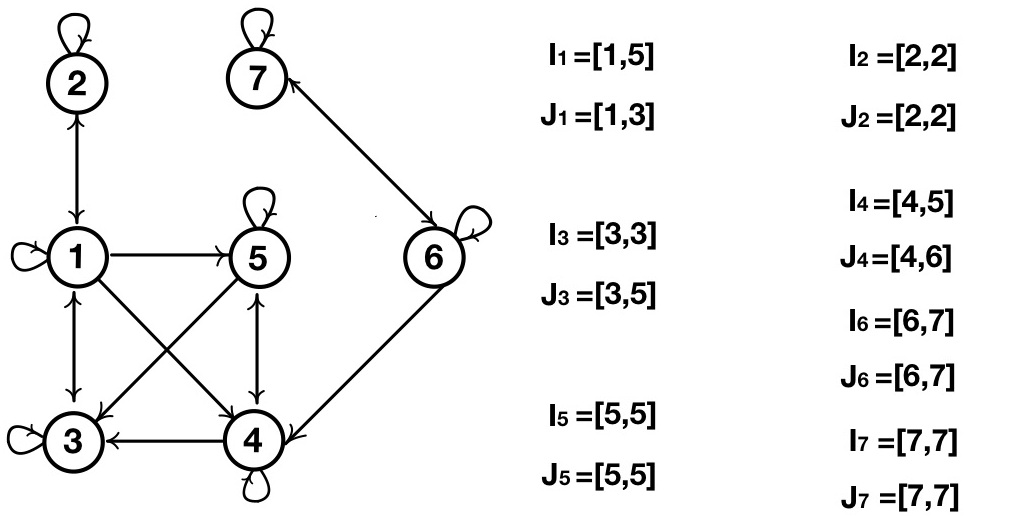
\includegraphics[width=0.75\textwidth]{recursos/capturas/MinOrdToIntGrph.jpg}
  \caption{Dada una digr\'afica reflexiva $G$ que admite un ordenamiento mínimo construimos la representaci\'on por pares de intervalos de $G$.}
  \label{fig:MinOrdToIntGrph}
\end{figure}

\begin{teorema}
    \label{teo:OrnMin_NoInvPair}
    Si $G$ tiene un par invertible, entonces $G$ no tiene un ordenamiento
    mínimo.
\end{teorema}

\begin{proof}
    Sea $u,v$ un {\color{malva} par invertible} en $G$. Por
    \cref{teo:PairDigrph} sabemos que $(u,v),(v,u)$ pertenecen a la misma
    componente conexa de la digr\'afica de pares $G^+$. Ahora, supongamos que
    $(x,y)(x', y')$ es una flecha de la digr\'afica de pares $G^+$. Supongamos
    que $<$ es un ordenamiento mínimo de $G$ y supongamos que $ u < v$. Entonces
    tambi\'en se tiene que $u'< v'$. Hagamos la prueba de este hecho. Como
    $(u,v)(u',v')\in E(G)$ entonces tenemos una de las siguientes dos
    situaciones, (i) $uu', vv'\in E(G)$ o $uv'\notin E(G) $ o (ii) $u'u, v'v \in
    E(G)$ o $ v'u \notin E(G) $. En el primer caso, veamos vía contradicci\'on
    que $u'<v'$.  Supongamos que $v'<u'$. Como $(u,v)(u',v')\in E(G)$ entonces
    $\min \{u,u' \}\min \{v,v' \}\in E(G)$, ya que por hip\'otesis tenemos un
    ordenamiento mínimo. Por otro lado, en el caso (i) tambi\'en tenemos la
    hip\'otesis $uv'\notin E(G)$, luego $\min \{u,u' \}\min \{v,v' \} \neq uv'$.
    Por lo que $\min \{u,u' \}=u'$ o $\min \{v,v' \}= v$. En el caso $\min
    \{u,u' \}=u'$, se tiene la siguiente cadena $v'<u'<u<v$ de donde $v'<u<v$ y
    dado que $vv'\in E(G)$, entonces por \cref{teo:OrdLnl} se tiene que $uv'\in
    E(G)$ lo cual es una contradicci\'on. Ahora en el caso en el que $\min
    \{v,v' \}= v$ se tiene la cadena $u<v<v'<u'$ de donde $u<v'<u'$ y dado que
    $uu'\in E(G)$ usando nuevamente \cref{teo:OrdLnl} $uv' \in E(G)$ lo cual es
    nuevamente una contradicci\'on. Ahora en el caso (ii) como $u'u, v'v \in
    E(G)$ entonces $\min \{u',v' \}\min \{u,v \}\in E(G)$, ya que tenemos un
    ordenamiento mínimo. En este caso tambi\'en tenemos que $v'u\notin E(G)$ así
    $\min \{u',v' \}  \min \{u,v \}\neq v'u$. Así las cosas $\min \{u',v' \}=u'$
    o $\min \{u,v \}=v$. En el caso en que $\min \{u',v' \}=u'$ se llega a
    $u'<v'$ que es precisamente lo que buscamos, mientras que el segundo caso
    $\min \{u,v \}=v$ no es posible, ya que en este caso $v<u$ pero por
    hip\'otesis $u<v$. Entonces $u = v$ lo cual no es posible. De todo lo
    anterior se concluye que $u'<v'$.    
    Retomando la prueba, consideremos $P$ el camino cerrado dirigido que
    contiene a $(u,v),(v,u)$, sigui\'endolo y haciendo uso de la nota anterior
    se llega a una contradicci\'on del tipo $u<v$ y $v<u$. Por lo que no es
    posible tener un ordenamiento mínimo en $G$ si hay presencia de un par
    invertible.
\end{proof}

\section{Digr\'aficas de intervalos ajustadas.}

En esta secci\'on enunciamos y probamos el teorema central de la tesis. 

\begin{teorema}
    Una digr\'afica reflexiva $G$ es una digr\'afica de intervalos ajustada si y
    solo si no tiene pares invertibles.
\end{teorema}

El teorema anterior lo probaremos vía las siguientes equivalencias.

 \begin{teorema}
     Sea $G$ una digr\'afica reflexiva, entonces las siguientes proposiciones
     son equivalentes.
\begin{enumerate}
  \item $G$ es una digr\'afica de intervalos ajustada.
  \item $G$ admite un ordenamiento mínimo.
  \item $G$ no tiene pares invertibles.
  \item Los v\'ertices de $G^+$ admiten una partici\'on en dos conjuntos $D, D'$
  tales que:
        \begin{enumerate}
            \item $(x,y)\in D $ si y solo si $ (y,x) \in D$
            \item $(x,y)\in D$ y $(x,y)$ domina a $(x',y')$ en $G^+$ implica que
            $(x',y')\in D$
            \item $(x,y), (y,z)\in D$ implica que $(x,z)\in D$
        \end{enumerate}
\end{enumerate}

\end{teorema}

\begin{proof}
  La equivalencia entre las primeras dos proposiciones se prob\'o en
  \cref{teo:DigrfIntAdj_OrdMin}. Por otro lado, mediante un uso de
  contrapositiva sobre \cref{teo:OrnMin_NoInvPair} se obtiene que la segunda
  proposici\'on implica la tercera. {\color{malva}Para probar que la cuarta
  proposici\'on implica la segunda, solo basta definir el ordenamiento $<$ como
  $u<v$ si y solo $(x,y) \in D$. } Finalmente procedamos a probar que la tercera
  proposici\'on implica la cuarta. Haremos la prueba de forma constructiva, es
  decir mediante un algoritmo veremos que asumiendo que $G$ es d\'ebilmente
  conexa (si no lo fuera, se puede aplicar el proceso a cada componente
  d\'ebilmente conexa) y suponiendo tambi\'en que $G$ no tiene pares
  invertibles, construiremos una partici\'on $\{D,D'\}$ de $V(G^+)$, que cumple
  (a), (b) y (c). Haciendo uso de \cref{teo:PairDigrph} se tiene que para cada
  componente fuertemente conexa $C$ de $G^+$ existe su componente fuerte
  revertida $C'$, es decir aquella tal que $(x,y)\in C $ si y solo si $(y,x)\in
  C'$. A las componentes de esta forma les llamaremos componentes fuertemente
  conexas acopladas o simplemente componentes acopladas. La partici\'on de
  $V(G^+)$ en $D,D'$ corresponder\'a a separar cada par de componentes acopladas
  $C$ y $C'$ de $G^+$. Los v\'ertices correspondientes a una componente $C$ los
  pondremos en $D$ y los v\'ertices revertidos los colocaremos en la componente
  $D'$. Al realizar el proceso, deberemos tener cuidado en no crear cadenas
  circulares, es decir una sucesi\'on de pares $(x_0,x_1)(x_1,x_2),\dots,
  (x_n,x_0)\in D$, ya que buscamos que se satisfaga (c) y la existencia de una
  cadena así implicaría $(x_0,x_0)\in D$, es decir $(x_0,x_0)\in G^+$ pero por
  construcci\'on en $G^+$ no hay v\'ertices de este estilo (diagonal). Al
  comenzar el algoritmo los conjuntos $D$ y $D'$ son vacíos. Decimos que una
  componente fuerte $C$ de $G^+$ es madura si no existen flechas desde $C$ a
  otra componente fuerte en $G^+ -D$. Entonces el paso general de nuestro
  algoritmo consistir\'a precisamente en colocar una componente fuerte madura
  $C$ en $D$ y colocar a la componente fuerte acoplada $C' $ en $D'$ ($C'$ no
  ser\'a necesariamente madura, pero s\'i se puede garantizar que no hay flechas
  desde $G^+ -D$ a $C'$, ver \cref{fig:FlechaRevertida}). Mostraremos que en
  cada paso del algoritmo, es posible añadir al menos una componente fuerte
  madura a $D$ sin crear cadenas circulares en $D$. Los conjuntos $D,D'$
  tendr\'an las siguientes propiedades, las cuales ser\'an ciertas de forma
  inicial. No existen cadenas circulares en $D$, cada componente fuerte de $G^+$
  pertenece enteramente a $D, D'$ o $V(G)-\{D,D' \}$, los pares en $D'$ son
  precisamente los pares revertidos de los pares en $D$; no hay flechas de $G^+$
  desde v\'ertices en $D$ a v\'ertices fuera de $D$ y no hay flechas en $G^+$
  desde v\'ertices fuera de $D'$ a un v\'ertice en $D'$. Al final del algoritmo,
  cada par $(x,y)$ con $x\neq y$ pertenecer\'a a $D$ o a $D'$ y así el conjunto
  final $D$ no tendr\'a cadenas circulares, por lo que se cumplir\'a $4$.
  Probemos que todas las propiedades anteriores se mantienen invariantes durante
  la ejecuci\'on del algoritmo. Supongamos por contradicci\'on que el $D$ actual
  no tiene cadenas circulares, pero que al añadir $C$, se crea una cadena en
  $C\cup D$, digamos $((x_0,x_1),(x_1,x_2),\dots, (x_n,x_0))$. Adem\'as,
  supongamos que es la primera vez que se obtiene la cadena durante la
  ejecuci\'on del algoritmo. Adicionalmente, sup\'ongase que no hay cadenas
  circulares mas cortas. Dado que por hip\'otesis no hay pares invertibles y que
  nunca se coloca un par y su par revertido en $D$, se tiene que $n\geq 2$. Con
  todo lo anterior, al menos un par de la cadena debe pertenecer a $C$ asumamos
  sin p\'erdida de generalidad que $(x_n,x_0)\in C$ (otros pares pueden estar
  tambi\'en en $C$). Bajo todas las condiciones anteriores, tenemos los
  siguientes dos casos.

  \textit{Caso 1.} Supongamos que en $G$ hay al menos una flecha entre un par de
  v\'ertices del conunto $\{ x_0,x_1,\dots,x_n \}$, digamos $(x_a,x_b)$. Veamos
  que esto implica que $\{ x_0,x_1,\dots,x_n \}$ es un clan de $G$. Para probar
  esto veamos las siguientes observaciones.
  \begin{enumerate}
    \item Si $x_j$ domina a $x_i$, entonces $x_{j-1}$ domina a $x_i$ en $G$.
    \item Si $x_j$ domina a $x_i$, entonces $x_j$ domina a $x_{i-1}$ en $G$.
  \end{enumerate}


Para probar la primera observaci\'on, notamos que, si $x_j$ domina a $x_i$ pero
$x_{j-1}$ no domina a $x_i$ en $G$, entonces $(x_{j-1},x_j)$ domina a
$(x_{j-1},x_i)$ en $G^+$. Dado que $(x_{j-1},x_j)$ pertence a $C\cup D$, la
pareja $(x_{j-1},x_i) $ debe pertenecer a $C\cup D$, ya que si $(x_{j-1},x_j)$
pertence a $C$ y $C$ es una componente fuertemente conexa, se sigue que
$(x_{j-1},x_i)\in C$. Ahora, si $(x_{j-1},x_j)$ pertence a $D$, como por
hip\'otesis se tiene que para toda flecha sale de un v\'ertice en $D$ tiene
cabeza en $D$, tenemos que $(x_{j-1},x_i)\in D$. En cualquier caso afirmamos que
existe una cadena circular m\'as pequeña en $C \cup D$. Veamos que siempre se
cumple una de las siguientes posibilidades: Si $i<j$, la cadena circular
tendr\'a una representaci\'on de la siguiente forma:
\[
  ( (x_0,x_1),(x_1,x_2),\dots, (x_{i-1},x_i), {\color{malva}(x_i,x_{i+1}),\dots,
  (x_{j-2},x_{j-1}),(x_{j-1},x_{j})}, \dots , (x_n,x_0))
\]
Como $(x_{j-1},x_i) \in C\cup D$, podemos ``sustituirlo'' en la cadena por el
v\'ertice $(x_{j-1},x_{j})$. Así, obtenemos la siguiente cadena, la cual en
efecto es mas corta, pues su longitud se corresponde con la longitud de la
subcadena en color malva.
\[
  ((x_i,x_{i+1}),\dots, (x_{j-2},x_{j-1}),(x_{j-1},x_i))
\]

Ahora, si $j<i$ la cadena circular tendr\'a una representaci\'on de la siguiente
forma:
$$( (x_0,x_1),\dots, (x_{j-2},x_{j-1}),
{\color{malva}(x_{j-1},x_j),(x_j,x_{j+1}) \dots,
(x_{i-1},x_{i})},(x_{i},x_{i+1}), \dots , (x_n,x_0))$$

Como $(x_{j-1},x_i) \in C \cup D$, podemos ``sustituirlo'' en la cadena por el
v\'ertice $(x_{j-1},x_{j})$. Así, obtenemos:
$$( (x_0,x_1),\dots, (x_{j-2},x_{j-1}), (x_{j-1},x_i),(x_{i},x_{i+1}), \dots ,
(x_n,x_0))$$ La cual es en efecto una cadena mas corta, ya que, en t\'erminos
simples $(x_{j-1},x_i)$ viene a sustituir toda la subcadena en color malva.

Ahora para probar la segunda observaci\'on, se tiene de forma an\'aloga que si
$x_j$ domina a $x_i$, pero $x_j$ no domina a $x_{i-1}$ en $G$, entonces
$(x_{i-1}, x_i)$ domina a $(x_{i-1}, x_j)$ en $G^+$, implicando nuevamente la
existencia de una cadena circular m\'as pequeña. Esto no es dif\'icil de
verificar mediante un par de esquemas como los usados para probar la primer
propiedad.

%%%%%%%%%%%%%%%%%%%%%%%%%%%%%%%%%%%%%%%%%%%%%%%%%%%%%%%%%%%%%%%%%%%%%%%%%%%%%%%%

Terminemos de ver que el hecho de tener una flechas entre dos v\'ertices de
$x_0,\dots,x_n$ nos lleva a que se tiene una gr\'afica completa en
$x_0,\dots,x_n$. Supongamos que $x_a$ domina a $x_b$ en $G$. La observaci\'on 1,
implica que todos los antecesores de $x_a$ dominan a $x_b$, es decir $x_{a-1},
x_{a-2},\dots, x_{b+1}$ dominan a $x_b$, observe el primer diagrama de la figura
123123. Ahora como $x_{b+1}$ domina a $x_b$ la propiedad 2, implica que
$x_{b+1}$ domina $x_{b-1}, x_{b-2},\dots,x_{b+2}$ esto es, domina a todos los
otros v\'ertices, ver el segundo diagrama de la figura 123123. Ahora usando
nuevamente la propiedad 1, tenemos que como $x_{b+1}$ domina a $x_{b-1}$
entonces $x_b$ domina a $x_{b-1}$, y aplicando la propiedad 2, se obtiene que
$x_b$ domina al resto de v\'ertices. Mediante la repetida aplicaci\'on de estas
propiedades sobre toso los v\'ertices, se puede concluir que los v\'ertices
$x_0,x_1,\dots,x_n$ inducen una gr\'afica completa en $G$. Finalmente veremos
que $C$ es una componente trivial, es decir consta de un solo v\'ertice,
supongamos que esto no es así es decir supongamos que en $C$ hay un v\'ertice
adicional del $(x_n,x_0)$, bajo estas hip\'otesis en la componente revertida
$C'$ debe tener a como v\'ertices a $(x_0,x_n)$ y a otro v\'ertice, supongamos
$(a,b)$, el cual no pertenece a $C\cup D$. Como $C'$ es conexa, se tiene que
$(x_0,x_n)$ domina a $(a,b)$, así podemos suponer que $x_0$ domina a $a$ en $G$,
$x_n$ domina a $b$ en $G$ y que $x_0$ no domina a  $b$ en $G$. Dado que $(a,b)$
no pertenece a $C\cup D$, entonces la pareja $(x_0,x_1)$ que pertenece a $C\cup
D$ no puede dominar a $(a,b)$ por lo que $x_1$ no domina a $b$ en $G$. Veamos
que $x_2$ tampoco puede dominar a $b$, si $x_2$  domina a $b$ en $G$ entonces
$(x_1,x_2)$ domina a $(x_0,b)$, recordemos que $x_1$ domina a $x_0$ porque
$x_0,x_1,\dots,x_n$ induce una gr\'afica completa, continuando, tenemos que a su
vez $(x_0,b)$ domina $(a,b)$ en $G^+$, pero esto no es posible ya que tendríamos
un camino dirigido que comienza en $C$ y termina fuera de $C\cup D$, por lo que
alguna flecha debe salir de $C\cup D$, que por hip\'otesis no puede pasar.
Nuevamente si $x_3$ domina a $b$ entonces $(x_2,x_3)$ domina a $(x_1,b)$ que a
su vez domina a $(a,b)$ y se llega a la misma contradicci\'on. De forma
an\'aloga, se puede probar que $x_n$ no domina a $b$, lo cual es falso. La
contradicci\'on de todo lo anterior surge de suponer que en $C$ hubo mas de un
v\'ertice. Así $C=\{ (x_n,x_0)\} $ y $C'=\{ (x_0,x_n)\}$. Con esta misma pruba
se muestra que $C'$ es una componente madura, pues no hay v\'ertices $(a,b)$ que
sean dominados fuera de $C\cup D$. Finalmente si $(x_n,x_0)$ y $(x_0,x_n)$
completan ambos una cadena circular con $D$, entonces en $D$ existía ya una
cadena circular. Por ejemplo 
$$  (y_0,y_1),(y_1,y_2),\dots, (y_k,x_0), (x_0,x_n), (x_n,x_0), (x_0,
y_{k+1}),\dots, (y_m,y_0) $$ Es una cadena que se forma con v\'ertices de $D$ y
con $(x_n,x_0)$ y $(x_0,x_n)$. Sin embargo, se puede formar la cadena 
$$  (y_0,y_1),(y_1,y_2),\dots, (y_k,x_0), (x_0, y_{k+1}),\dots, (y_m,y_0) $$ Que
consta de v\'ertices de $D$. 

Pasemos ahora a probar el segundo caso, en este caso suponemos que
$x_0,x_1,\dots,x_n$ es un conjunto independiente en $G$. Probaremos un par de
lemas auxiliares. 

\begin{lema}
  \label{lem:Sustitucion}
  Sea $x_0,x_1,\dots,x_n $ un conjunto independiente en $G$. Supongamos que $p$
  es un v\'ertice de $G$ distinto de $x_0,x_1,\dots,x_n$, el cual domina a
  $x_{i+1}$ pero no a $x_i$. Entonces $(x_0,x_1),\dots,
  (x_i,p)(p,x_{i+2}),\dots, (x_n,x_0)$ es tambi\'en una cadena circular creada
  al mismo tiempo.
\end{lema}
\begin{proof}
  Del hecho de que $(x_ix_{i+1})$ domina a $(x_i,p)$ en $G^+$ y dado que
  $(x_i,x_{i+1})$ pertenece a $C\cup D$ se debe tener que $(x_i,p)$ debe
  pertenecer tambien a $C\cup D$. Adem\'as, dado que $x_{i+1}$ no domina o es
  dmoinado por $x_{i+2}$ en $G$, tambi\'en debemos tener que $(x_{i+1},x_{1+2})$
  domina a $(p,x_{+2})$ cuando $(p,x_{i+2})$ est\'a en $C\cup D$. En
  conclusi\'on vemps que cualquier v\'ertice $p$ podemos reemplazarlo por
  $x_{i+1}$ en la cadena circular $(x_0,x_1),(x_1,x_2),\dots , (x_n,x_0)$
\end{proof}

\begin{lema}
  \label{lem:Completa}
  Supongamos que el conjunto $x_0,x_1,\dots,x_n$ es un conjunto independiente:
  \begin{enumerate}
    \item Si $p$ es un v\'ertice de $G$ distinto de $x_0,x_1,\dots,x_n$ el cual
    domina a $x_j$ y $x_k$, con $j\neq k$, entonces $p$ domina a cada $x_i$.

    \item Si $p$ es un v\'ertice de $G$ distinto de $x_0,x_1,\dots,x_n$ el cual
    es dominado por $x_j$ y $x_k$, con $j\neq k$, entonces $p$ es dominado por
    cada $x_i$.

    \item Si $p$ es un v\'ertice de $G$ distinto de $x_0,x_1,\dots,x_n$ el cual
    domina a $x_j$ y es dominado por $x_k$, con $j\neq k$, entonces $p$ es
    domina y es dominado por cada $x_i$.
  \end{enumerate}

\end{lema}

\begin{proof} 
  Si $p $ domina a $x_{i+1}$ pero no a $x_i$ usando \cref{lem:Sustitucion}
  tenemos que $p$ puede reemplazar a $x_{i+1}$ en la cadena circular. Ahora,
  $x_j$ o $x_k$, alguno de los dos es distinto de $x_{i+1}$ (ya que
  $x_0,x_1,\dots,x_n$ es independiente). Entonces estamos en el caso en el que
  tenemos una cadena donde hay al menos una flecha, luego por el caso 1, se
  llega a que tenemos una gr\'afica completa. Los otros dos puntos pueden
  probarse de una manera similar.
\end{proof}  

Afirmamos ahora que en la cadena circular $(x_0,x_1),(x_1,x_2),\dots ,
(x_n,x_0)$ hay a lo mas una pareja en $C$, supongamos que es $(x_n,x_0)$ y el
resto de parejas pertenecen a $D$. Supongamos que esto no es así, es decir que
adem\'as de $(x_n,x_0)$ hay otra pareja $(x_i,x_{i+1})$ en $C$ $i\neq n$ y sea
$P$ un camino dirigido en $C$ de $(x_n,x_0)$ a $(x_i,x_{i+1})$. Sea $(p,q)$ el
penúltimo v\'ertice en este camino y supongamos sin p\'erdida de generalidad que
$px_i,qx_{i+1}\in E(G), px_{i+1}\notin E(G)$. Por \cref{lem:Completa} $p$ no
puede dominar a ningún otro $x_j$ ya que llegariamos a que domina a dos
v\'ertices y por ende dominaría a todos e particular a $x_{i+1}$. Ahora, $q$ no
domina a $x_i$, de hecho si $q$ domina a $x_i$ nuevamente por
\cref{lem:Completa} tendremos que $q$ domina a todos los $x_i$, esto es una
contradicci\'on ya que se llega a que $(p,q)$ domina a $(x_i,x_{i+2})$ en $G^+$
lo que nos dice que $(x_i,x_{i+2})$ pertenece a $C\cup D$ y así tendemos una
cadena circular mas pequeña en $H$. Tal como se muestra abajo:
$$ (x_,x_1), \dots , (x_{i-1},x_i ), {\color{malva} (x_i,x_{i+1}),
(x_{i+1},x_{i+2})},(x_{i+2},x_{i+3}), \dots , (x_n,x_0) $$
$$ (x_,x_1), \dots , (x_{i-1},x_i ), {\color{malva}
(x_i,x_{i+2})},(x_{i+2},x_{i+3}), \dots , (x_n,x_0) $$ Por lo tanto $q$ no
domina a $x_i$. Mediante una doble aplicaci\'on d\cref{lem:Sustitucion}
concluimos que $x_i,x_{i+1}$ pueden ser reemplazados por $p,q$ respectivamente
en la cadena circular en $G$. Continuando de esta forma, podemos reemplazar
$(p,q)$ por el par previo en el camino $P$, hasta obetener el par $(p',q')$ el
cual es el primero en aparecer en el camino que es distinto de $(x_n,x_0)$. Dado
que $x_0$ es adyacente a $q'$, regresamos al caso 1.

Así en efecto en la cadena $(x_0,x_1),(x_1,x_2),\dots,(x_n,x_0)$ tiene solamente
el par $(x_n,x_0)$ en $C$ y cualquier otra cadena en $C\cup D$ debe tener
exactamente un par en $C$. Ahora asumimos que nuestra cadena circular minimiza
la suma de la longitud de la distancia entre los vértices $x_0,x_1,\dots ,x_n$
en la gráfica subyacente de $G$.

La digráfica $G$ resulta tener una estructura muy especial. Afirmamos que en
esta situación existe un conjunto no vac\'io $K$ de vértices de $G$ tales que
$G-K$ tiene componentes d\'ebiles $C_1,c_2,\dots,C_m$ donde $x_i\in C_i$ con
$i=1,\dots,n$ y tal que si $p\in K$ domina un vértice en $C_i$ entonces $p$
domina todos los vértices de $C_i$, mas aún si $x'_0,x'_1,\dots,x'_n$ son
cualesquiera vértices con $x'_i\in C_i$ entonces
$(x'_0,x'_1),(x'_1,x'_2),\dots,(x'_n,x'_0)$ es también una cadena circular. El
conjunto $K$ corresponde a todos los vértices de $G$ que dominan a cada $x_i$ o
que son dominados por cada $x_i$. Recordando \cref{lem:Completa} se tiene que
para que un $p$ pertenezca a $K$ basta dominar o ser dominado por dos elementos
de $\{x_0,x_1,\dots,x_n \}$. Ahora, debe existir un $p\in K$ ya que estamos
asumiendo que la cadena minimiza la suma de la longitud de las distancias entre
los v\'ertices, es decir si no existe un $p$ el cual domina (o es dominado) por
al menos dos elementos de $\{x_i \}_{i=1} ^n$, entonces eso quiere decir que
todo $p$ v\'ertice de $G-\{x_i\}_{i=1} ^n$ domina a un único $x_i$, mas aún
domina a $x_i$ y no domina a $x_{i-1}$. Entonces, haciendo uso
d\cref{lem:Sustitucion}, obtenemos una cadena circular mas pequeña, lo que
contradice el hecho de haber tomado una cadena que minimiza la suma de las
longitudes.

El mismo argumento muestra que dos v\'ertices distintos $x_j, x_k$ no pueden
estar en la misma componente débil $C_i$ de $G - K$, ya que se demostró que
cualquier camino que conecta $x_j$ con $x_k$ contiene un vértice de $K$. Por lo
tanto, podemos numerar los componentes de manera que $C_i$ contenga a $x_i$ para
$i = 1, 2, \dots, n$. (Puede haber componentes adicionales $Ci $ con $i = n + 1,
\dots , m$.) Ahora, \cref{lem:Sustitucion} implica que cada $x_i$ puede ser
reemplazado por cualquier vecino en $C_i$; así, cualquier vértice de $C_i$ puede
tomarse como $x_i$. De esta manera, cada $p \in K$ que domina un vértice en
$C_i$ también domina todos los vértices en $C_i$, y de manera similar para los
vértices $p$ dominados por un vértice en $C_i$.

Esto crea una situación en la que cualquier par $(y, y')$ en la componente
fuerte $C$ de $G^+$ que contiene $(x_n, x_0)$ debe satisfacer $y \in  C_n, y'
\in C_0$. Esto implica fácilmente que la componente fuerte $C$ no tiene aristas
que ingresen desde el exterior, y por lo tanto, la componente fuerte $C'$ junto
con $C$ son maduras. $C'$ no puede completar una cadena circular con $D$. De lo
contrario, el par $(x_0, x_n)$ también completaría una cadena circular por el
mismo argumento. Por lo que, tanto $(x_0, x_n)$ como $(x_n, x_0)$ completan
una cadena circular con $D$, de donde se sigue que $D$ ya debe contener una
cadena circular, lo cual es una contradicción.

Por supuesto, si la adición de $C'$ no crea una cadena circular, entonces
agregamos $C '$ a $D$ y $C$ a $D'$.
\end{proof}